\begin{abstract}
Every database system contains a query optimizer that performs query rewrites.
Unfortunately, developing query optimizers remains a highly challenging task.
Part of the challenges comes from the intricacies and rich features of query 
languages, which makes reasoning about the correctness of SQL rewrite rules difficult.

In this paper, we built VeriCQ, a SMT based tool that automatically checks 
the correctness of conjunctive SQL query rewrite rules. To provide 
confidence in the VeriCQ's results, it is formally verified against a semantics of
SQL called \sem~\cite{hottsql} in the Coq proof assistant.

In our evaluation, we show that the use of an SMT
solver can improve the performance of query equivalence checking by
orders of magnitude, over a naive implementation.
\end{abstract}

\section{Introduction}

From purchasing plane tickets to browsing social networking websites,
we interact with database systems on a daily basis. 
Every database system consists of a query optimizer that
takes in an input query and 
determines the best program, also called a query plan, to execute 
in order to retrieve the 
desired data. Query optimizers typically consists of two components:
a query plan enumerator that generates query plans that are semantically
equivalent to the input query, and a plan selector that chooses 
the optimal plan from the enumerated ones to execute
based on a cost model.

The key idea behind plan enumeration is to apply {\em rewrite rules}
that transform a given query plan into another one, hopefully one with
a lower cost.  While numerous plan rewrite rules have been proposed
and implemented, unfortunately designing such rules remains a highly
challenging task.  For one, rewrite rules need to be {\em semantically
  preserving}, i.e., if a rule transforms query plan $Q$ into $Q'$,
then the results (i.e., the relation) returned from executing $Q$ must
be the same as those returned from $Q'$, and this has to hold for {\em
  all} possible input database schemas and instances.  Obviously,
establishing such proof for any non-trivial query rewrite rule is not
an easy task.

Coupled with that, the rich language constructs and subtle semantics of
SQL, the de facto programming language used to interact with relational 
database systems, 
only makes the task even more difficult.
As a result, while various rewrite rules
have been proposed and studied extensively 
in the data management research community~\cite{MumickFPR90SIGMOD, Muralikrishna92VLDB, LevyMS94VLDB, SeshadriHPLRSSS96SIGMOD},
not many of these have been formally verified. This has unfortunately 
led to dire consequences as incorrect query results have been returned 
from widely-used database systems due to unsound rewrite rules, and 
such bugs can often go undetected for extended periods of time
\cite{GanskiW87SIGMOD, MySQLBug, PostgresBug}.

In this paper we describe a system called VeriCQ to automatically and formally verify SQL query rewrite rules.
Such a tool is impossible to build for arbitrary rewrite rules, as SQL query equivalence is an 
undecidable problem, but we provide a tool that does this for rewrite rules involving 
a subset of SQL queries called \emph{conjunctive queries}.

To efficiently verify SQL rewrite rules, VeriCQ reduces rewrite problems to the domain of
a highly optimized SMT solver like Z3.
%
To provide confidence in the VeriCQ's results, it is formally verified against a semantics of
SQL called \sem~\cite{hottsql} in the Coq proof assistant. 

VeriCQ is verified using the \SpaceSearch~\cite{SpaceSearch} library, which enables the verification of 
SMT solver based tools. 
%
Using \SpaceSearch, we built VeriCQ in Coq, using operations from the
\SpaceSearch library to call a solver.
%
We then verified that the low-level results from solver calls can
be lifted to the correctness of SQL query rewrite rules.
%
Once verified, we extracted (compiled) VeriCQ to Racket,
where the \SpaceSearch interface is instantiated with an efficient
implementation that uses an SMT solver.

In our evaluation, we show that the use of an SMT
solver can improve the performance of query equivalence checking by
orders of magnitude, over a naive implementation.


\section{VeriCQ}

\begin{figure}
\begin{small}
\textbf{Rewrite Rule}:
\begin{flalign*}
\quad\; & \SelectFromWhere{\Star}{(\UNIONALL{R}{S})}{\pred} \quad \equiv & \\
        & \UNIONALL{(\SelectFromWhere{\Star}{R}{\pred})} & \\
        & {(\SelectFromWhere{\Star}{S}{\pred})} &
\end{flalign*}

\textbf{\sem Denotation}:
\begin{flalign*}
% \Rightarrow & \lambdaFn{t}{\denote{\UNIONALL{A}{B}} \; t \times \denote{\pred} \; t} \quad= & \\ 
% %
% & \lambdaFn{t}{\denote{\SelectFromWhere{\Star}{A}{\pred}} \; t +
%                \denote{\SelectFromWhere{\Star}{B}{\pred}} \; t} & \\
% %%
\Rightarrow & \lambdaFn{t}{(\denote{R} \; t + \denote{S} \; t) \times \denote{\pred} \; t}
%
\equiv & \\
%
& \lambdaFn{t}{\denote{R} \; t \times \denote{\pred} \; t + \denote{S} \; t \times \denote{\pred} \; t} &
%
\end{flalign*}

\textbf{\sem Proof}:
Apply distributivity of $\times$ over $+$.
\end{small}
\caption{Proving a rewrite rule using \sem.
Recall that \texttt{UNION ALL} means bag-union in SQL, which in \sem
is translated to addition of tuple multiplicities in the two input relations.
}
\label{fig:union-slct}
\end{figure}

The basic datatype in SQL is a {\em relation}, 
which is defined as bag of \emph{tuples}.
Each tuple in the bag must be of the same type, which
is defined by a relation's {\em schema}.
The schema defines the number of elements per tuple, 
and the name and type of each element.

A SQL query takes several input
relations and returns a new output relation. Consider, for example,
a relation $R$, which stores a company's employees and their age. 
$R$ has schema $\{\nameCol : \sqlString; \; \texttt{age} : \sqlInt)\}$
and value $\{(``Alice'', 25),(``Bob'',40),(``Bob'',50)\}$.
%
The SQL query that selects all employees without their age is:
%
\begin{flalign*}
  \SelectFrom{\nameCol}{R}
\end{flalign*}
%
It returns the bag $\{(``Alice''),(``Bob''),(``Bob'')\}$.  

Green \etal's semantics~\cite{k-relations} represent relations as functions that
map every tuple to a natural number that indicates how many times it appears
in the relation. With this semantics,
all queries can be defined in terms of operations on the natural numbers.
We use the notation $\denote{q}$ to define the meaning of
(denote) the SQL query $q$. Consider, for example:

\begin{align*}
  & \denote{\UNIONALL{q_1}{q_2}} =  \lambdaFn{\tuple}{\denote{q_1} \; \tuple+\denote{q_2} \; \tuple} \\ 
  & \denote{\SelectFromWhere{\Star}{q_1}{\pred}} = \lambdaFn{\tuple}{\denote{q_2} \; \tuple \times \denote{\pred} \; \tuple} \\
\end{align*}

The query $\UNIONALL{q_1}{q_2}$ combines 
the tuples in the relation returned by the query $q_1$ with 
the tuples in the relation returned by the query $q_2$ (without removing duplicates).
The result is a relation,
and thus a function, that maps every tuple $\tuple$ to the number of times 
that tuples appears in $q_1$ plus the number of times that the tuple appears in $q_2$.

The query $\SelectFromWhere{\Star}{q}{\pred}$ removes all the tuples, from the
relation returned by the query $q$ for which the predicate $\pred$ does not hold. We denote the predicate
as a function $\denote{\pred}$ that maps a tuple to $1$ if the predicate holds,
and $0$ otherwise. The query multiplies the relation with the
predicate to achieve the desired effect (i.e. $n \times 1 = n$ and $n \times 0 = 0$).

To prove that two
SQL queries are equal one has to prove that, forall tuples, the two natural number expressions
are equal. 
% which is much simpler than the inductive proof required under the list semantics.
For example, Fig.~\ref{fig:union-slct}
shows how we can prove that selections distribute over unions, by
reducing it to the distributivity of $\times$ over $+$. 
% while
% Fig.~\ref{fig:magic-distinct} shows the proof of the equivalence for
% $\texttt{Q2} \equiv \texttt{Q3}$.

\begin{figure*}
\centering
\begin{tabular}{|l|l|l|l|l|} \hline
 & Containment (Set)  & Containment (Bag) & Equivalence (Set) &  Equivalence (Bag) \\ \hline 
Conjunctive Queries & NP-Complete \cite{sql-hardness-cq-set} & Open & NP-Complete \cite{sql-hardness-cq-set}  &  Graph Isomorphism \cite{sql-hardness-cq-bag-equality} \\ \hline
% 
Union of Conjunctive Queries & NP-Complete \cite{sql-hardness-cqunion-set}  & Undecidable \cite{sql-hardness-cqunion-bag-containment}  & NP-Complete \cite{sql-hardness-cqunion-set}  & Open \\ \hline 
%
Conjunctive Query with $\neq$, $\geq$, and $\leq$ & 
$\Pi_2^p$-Complete \cite{sql-hardness-cqex-set} & Undecidable  \cite{sql-hardness-cqex-bag} &  $\Pi_2^p$-Complete  \cite{sql-hardness-cqex-set}  & Undecidable \cite{sql-hardness-cqex-bag}  \\ \hline
%
First Order (SQL) Queries & Undecidable \cite{sql-hardness-first-order} & Undecidable  \cite{sql-hardness-first-order} & Undecidable  \cite{sql-hardness-first-order} & Undecidable  \cite{sql-hardness-first-order} \\ \hline
\end{tabular}
\caption{Complexities of Query Containment and Equivalence.}
\label{fig:complexity}
\end{figure*} 

The equivalence of two SQL queries is in general
undecidable~\cite{sql-hardness-first-order}. Figure~\ref{fig:complexity}
shows the complexities of deciding containment and equivalence of
subclasses of SQL.
%
The most well-known subclass are conjunctive queries, which are of the
form \texttt{SELECT DISTINCT $p$ FROM $q$ WHERE $b$}, where $p$ is a
sequence of arbitrarily many attribute projections, $q$ is the cross
product of arbitrarily many input relations, and $b$ is a conjunct
consisting of arbitrarily many equality predicates between attribute
projections.
%
The \sem paper provides a tactic to automatically prove
the equivalence of conjunctive queries in \sem, using Coq's support
for automating deductive reasoning (with \emph{Ltac}).

However, this approach has two major drawbacks. 
1) The tactic is slow because it performs brute-force search over an exponentially large space, and
   because it is implemented in the high-level interpreted Ltac language.
2) The tactic may generate a proof for a particular rewrite rules correctness, but there
   are no guarantees that the tactic will always terminate and generate a proof. 

We re-implement this tactic as a Coq program (a
function that literally returns a proof that the two queries are equal)
using the \SpaceSearch
framework, which will eliminate the drawbacks of the tactic approach:
1) the decision procedure will be fast as it can be extracted to an SMT query, and
2) it will be verified.
%
We can potentially also implement a decision procedure for other
subclasses mentioned in~\ref{fig:complexity} that are NP-Complete and
that can thus be reduced to a SAT problem.


\section{SpaceSearch}

VeriCQ uses the \SpaceSearch library to verify SQL query rewrites. 
This section describes \SpaceSearch, a framework for verifying any solver-aided 
tools in Coq. Solver-aided tools written against \SpaceSearch can be
translated to a solver-aided host language (e.g., Rosette~\cite{rosette:onward13} and Smten~\cite{smten}), which 
uses SMT solvers for efficient verification of (finite) programs.

\begin{figure}
\begin{lstlisting}
$\ssSpace : Type \rightarrow Type$ %\textnormal{ \hfill --- sets whose members are of type $A$}%
$\ssFree_A : \ssSpace(A)$ %\textnormal{ \hfill --- all terms inhabiting $A$}%
$\ssEmpty_A : \ssSpace(A)$ %\textnormal{ \hfill --- an empty space}%
$\ssSingle_A : A \rightarrow \ssSpace(A)$ %\textnormal{ \hfill --- create a singleton space}%
$\ssUnion_A : \ssSpace(A) \rightarrow \ssSpace(A) \rightarrow \ssSpace(A)$ %\textnormal{ \hfill --- merge two spaces}%
$\ssBind_{A,B} : \ssSpace(A) \rightarrow (A \rightarrow \ssSpace(B)) \rightarrow \ssSpace(B)$
$\ssSearch_A : \ssSpace(A) \rightarrow A \cup \bot$%\textnormal{\hfill --- returns an element in $A$; $\bot$ if empty}%

$\denote{\ssSpace(A)} = Set(A)$
$\denote{\ssFree_A} = \{a  \mid  a : A\}$
$\denote{\ssEmpty_A} = \emptyset$
$\denote{\ssSingle_A(a)} = \{a\}$
$\denote{\ssUnion_A(s,t)} = \denote{s} \cup \denote{t}$
$\denote{\ssBind_{A,B}(s,f)} = \bigcup_{a \in \denote{s}} \denote{f(a)}$
$\denote{\ssSearch_A(s)} =$ if $\denote{s} = \emptyset$ then $\bot$ else $\axiomOfChoice(\denote{s})$

$\ssEmpty_A() \triangleq$ (lambda (v) (assert false))
$\ssSingle_A(a) \triangleq$ (lambda (v) a)
$\ssUnion_A(s,t) \triangleq$ (lambda (v) 
  (if (symbolic-bool) (s v) (t v)))
$\ssBind_{A,B}(s,f) \triangleq$ (lambda (v) (f (s v) v))
$\ssSearch_A(s) \triangleq$ (search s)      ;; calls Rosette solver

\end{lstlisting}
\caption{\SpaceSearch DSL\@. 
$\ssSpace$ forms a monad with $\ssSingle$ and $\ssBind$.
$\ssBind(s,f)$ maps the function $f$ over every element in $s$ and unions the results.
For Rosette to execute Coq terms written against this interface, the Coq terms
must be extracted to Racket as shown at the bottom of the figure.}
\label{fig:rosette}
\end{figure}

\SpaceSearch does not expose a full solver-aided host language directly to Coq.
Instead, \SpaceSearch exposes a monadic domain-specific language (DSL).
\SpaceSearch is
inspired by Smten, and is based on constructing search
spaces of values to be explored by the underlying SMT solver. \SpaceSearch is defined in \cref{fig:rosette}, and includes a
number of functions for building spaces and a search function for
finding a member of a space if one exists.

In Coq, the \SpaceSearch functions are denoted in terms of
sets.
The $\ssFree_A$ set, which must
be implemented for every type $A$ separately (using the provided space-building  
functions), %must return a set which
contains every member of a finite type $A$. This set  cannot be implemented
for infinite types like $\nat$.

% Rosette using Coq's extraction mechanism. 

\SpaceSearch can run programs written against this interface by 
extracting the Coq terms to Rosette.
Rosette implements symbolic boolean and integer 
values, assertions, and a \lstinline{search} function, which takes as input an
expression and tries to find a concrete assignment to any symbolic
values in that expression that does not violate any assertions. The
\lstinline{search} function works by translating the input expression
into an SMT formula and solving it with an off-the-shelf  
SMT solver.  Coq's built-in extraction facility translates
user-defined functions directly to Racket syntax (which is also Rosette's syntax), but the extractions
for particular functions can be overridden. \SpaceSearch does this for
the functions listed in \cref{fig:rosette}; each set-construction
function is translated to an equivalent term that uses Rosette's
assertions and symbolic booleans.  The $\ssSearch$ function, meanwhile, is extracted
to a call to Rosette's \lstinline{search} function.

\SpaceSearch supports extraction of search spaces to both \emph{concrete} and \emph{symbolic} expressions in 
Rosette. 
When
the \SpaceSearch functions are extracted to concrete expressions, spaces are
enumerated explicitly; for instance, $\ssBind(s,f)$ is
extracted to \lstinline{flatten (map $f$ $s$)}.  When they are extracted to symbolic expressions, 
their enumeration is performed symbolically, by the underlying SMT solver.  
Concrete extraction is best suited for small to medium-sized search spaces $s$, such as all routers in
a network, and complex functions $f$, such as checking whether a policy holds
for a router, enabling trivial parallelization by distributing the application of $f$ with
elements in $s$ to nodes in a cluster.  Symbolic extraction, in contrast, works best for 
simple functions $f$ (such as $\lambda n. n \neq
892412$) applied to large search spaces $s$ (such
as the 32 bit integers). 
%
By extracting a program's outer binds with medium-sized search spaces to
concrete expressions, and extracting an algorithm's inner binds with large search spaces to
symbolic expressions, users of \SpaceSearch can get the best of both
worlds: algorithms that explore large search spaces using both parallelism and
solver technology.

\begin{figure}
\begin{lstlisting}
$\ssFree_\Boolean : \ssSpace(\Boolean)$
$\ssFree_\Boolean := \ssUnion(\ssSingle(\true), \ssSingle(\false))$

$\idempotent : \ssSpace(\Boolean \times \Boolean)$
$\idempotent :=$
  $x \leftarrow \ssFree_\Boolean;$ $y \leftarrow \ssFree_\Boolean;$
  if $(x \oplus y \oplus y = x)$ then $\ssEmpty$ else $\ssSingle(x,y)$

$\xorResult : (\Boolean \times \Boolean) \cup \bot$
$\xorResult := \ssSearch(\idempotent)$
\end{lstlisting}
\caption{
\SpaceSearch Example. $\idempotent$ is the $\ssSpace$ which contains all examples for
which the XOR operation on boolean values is \emph{not} idempotent. When the space is
passed to Rosette via $\ssSearch$, the result is $\bot$ because there is no
counterexample for the idempotence of XOR. The notation $x \leftarrow s; f$
means $\ssBind(s,\lambda x. f)$.
}
\label{fig:rosette-example}
\end{figure}

\cref{fig:rosette-example} shows an example of a simple program in the \SpaceSearch DSL. The program verifies the idempotence of
the XOR operation on boolean values. The $\ssBind$ operations can be extracted 
to either concrete or symbolic expressions.


% Further, we require algorithms that target Rosette as a solver to be of the
% form $\verify (s_0 \in S_0; s_1 \in S_1; \dots; \return(f(s_0,s_1,\dots))$,
% which can be translated to Rosette by replacing each monadic bind with a
% symbolic variable declaration, and the return with an assertion. Algorithms
% in this form can be interpreted as
% $\verify \{f(s_0,s_1,\dots) | s_0 \in S_0, s_1 \in S_1, \dots \}$.


\section{Evaluation}

In our evaluation, we show that the use of an SMT
solver can improve the performance of query equivalence checking by
orders of magnitude, over a naive implementation. \Cref{fig:eval}
shows our evaluation of VeriCQ.

We evaluate 


\begin{figure*}
\begin{flalign*}
\quad\; & \SelectFromWhere{x_0.a}{R \; \texttt{AS} \; x_0, R \; \texttt{AS} \; x_1, R \; \texttt{AS} \; x_2, R \; \texttt{AS} \; x_3}{x_0.a = x_1.a  \; \texttt{AND} \; x_1.a = x_2.a \; \texttt{AND} \; x_2.a = x_3.a} \quad \equiv & \\
        & \SelectFromWhere{x_0.a}{R \; \texttt{AS} \; x_0, R \; \texttt{AS} \; x_1, R \; \texttt{AS} \; x_2, R \; \texttt{AS} \; x_3}{x_1.a = x_2.a  \; \texttt{AND} \; x_2.a = x_3.a \; \texttt{AND} \; x_0.a = x_1.a} &
\end{flalign*}
\caption{Proving a rewrite rule using \sem.
Recall that \texttt{UNION ALL} means bag-union in SQL, which in \sem
is translated to addition of tuple multiplicities in the two input relations.
}
\label{fig:union-slct}
\end{figure*}


\begin{figure}
\centering
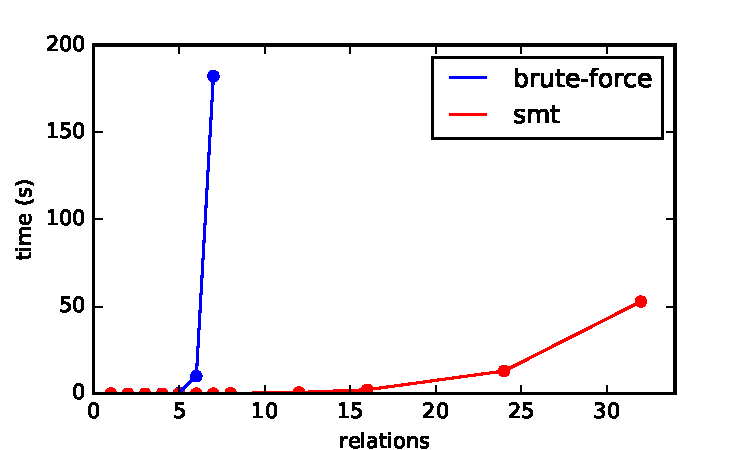
\includegraphics[width=\columnwidth]{eval/eval.pdf}
\caption{Evaluation of Naive vs SMT based rewrite rule verification.}
\label{fig:eval}
\end{figure}

